\documentclass[handout]{beamer}
\usepackage[T1]{fontenc}
\usepackage[utf8]{inputenc}
\usepackage{lmodern}
\usepackage[italian]{babel}
\usepackage{mathrsfs}
\usepackage{cancel}
\usepackage{multicol}

\title{La misurazione}
\author{Mattia Cozzi}
\date{a.f.~2024/2025}
%\documentclass[handout]{beamer}     %usare questa classe per generare l'handout
%\usepackage{pgfpages}   %per mostrare più quadri nella stessa pagina
%\pgfpagesuselayout{4 on 1}[a4paper,border shrink=5mm,landscape]
\usetheme{Singapore}
%\useoutertheme[left]{sidebar} %elementi intorno alle diapositive
\setbeamercovered{dynamic} %modifica l'aspetto del testo grigetto delle diapositive future. Argomenti: invisible/transparent/dynamic

\usecolortheme{orchid}


\theoremstyle{plain}
\newtheorem{teorema}{Teorema}

\usepackage{tikz}
\usepackage{circuitikz}

\usepackage{pgf,pgfplots,graphicx}
\usetikzlibrary{angles,quotes,arrows,shapes,decorations.markings}
\pgfplotsset{compat=1.15}
\usepgfplotslibrary{units,fillbetween} % to add units easily to axis


\def\angolo[#1](#2)(#3:#4:#5)% Syntax: [draw options] (center) (initial angle:final angle:radius)
    { \draw[#1] ($(#2)+({#5*cos(#3)},{#5*sin(#3)})$) arc (#3:#4:#5); }


\begin{document}

\begin{frame}
  \titlepage
\end{frame}





\begin{frame}
\frametitle{Contenuti}
\tableofcontents
\end{frame}


\section{Premessa}




\begin{frame}
\frametitle{A cosa serve la matematica nel mondo?}
\begin{quote}
  La filosofia è scritta in questo grandissimo libro che continuamente ci sta aperto innanzi a gli occhi (io dico l'universo), ma \alert<1>{non si può intendere se prima non s'impara a intender la lingua, e conoscer i caratteri, ne' quali è scritto}.\pause
  
  ~

  \alert<2>{Egli è scritto in lingua matematica}, e i caratteri son triangoli, cerchi, ed altre figure geometriche, senza i quali mezzi è impossibile a intenderne umanamente parola; senza questi è un aggirarsi vanamente per un oscuro laberinto.
  \begin{flushright}
    Galileo Galilei, \emph{Il Saggiatore}, 1623 
  \end{flushright}
\end{quote}
\end{frame}




\begin{frame}
\frametitle{Parti dell'unità}
Ci sono alcuni \alert{numeri decimali speciali}:

\[ 0,1 \qquad \qquad 0,01 \qquad \qquad 0,001 \]\pause

Questi numeri indicano:
\begin{itemize}
  \item la \alert{decima parte} dell'unità (1 parte su 10);\pause
  \item la \alert{centesima parte} dell'unità (1 parte su 100);\pause
  \item la \alert{millesima parte} dell'unità (1 parte su 1000);
\end{itemize}
\end{frame}



\begin{frame}
\frametitle{Decimi}
\begin{columns}
  \begin{column}{0.3\textwidth}
  \begin{figure}
    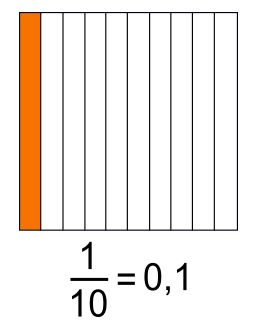
\includegraphics[width=\columnwidth]{img/decimi1.png}
  \end{figure}    
  \end{column}
  \begin{column}{0.6\textwidth}
    Dalla figura, possiamo capire che \alert{dieci decimi sono un'unità}.

    ~
  \end{column}
\end{columns}
\begin{figure}
  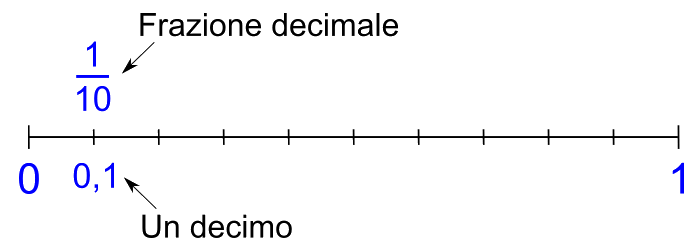
\includegraphics[width=.8\columnwidth]{img/decimi2.png}
\end{figure}
\end{frame}




\begin{frame}
\frametitle{Centesimi}
\begin{columns}
  \begin{column}{0.3\textwidth}
  \begin{figure}
    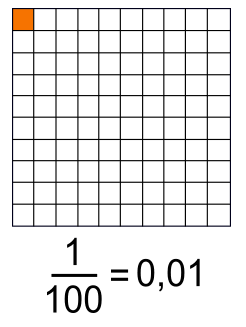
\includegraphics[width=\columnwidth]{img/centesimi1.png}
  \end{figure}    
  \end{column}
  \begin{column}{0.6\textwidth}
    Dalla figura, possiamo capire che \alert{cento centesimi sono un'unità}.

    ~
  \end{column}
\end{columns}
\begin{figure}
  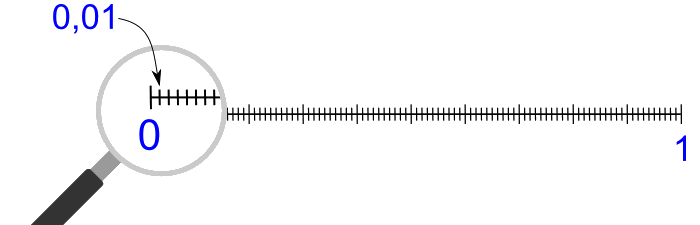
\includegraphics[width=.8\columnwidth]{img/centesimi2.png}
\end{figure}
\end{frame}



\begin{frame}
\frametitle{Millesimi}
\begin{figure}
  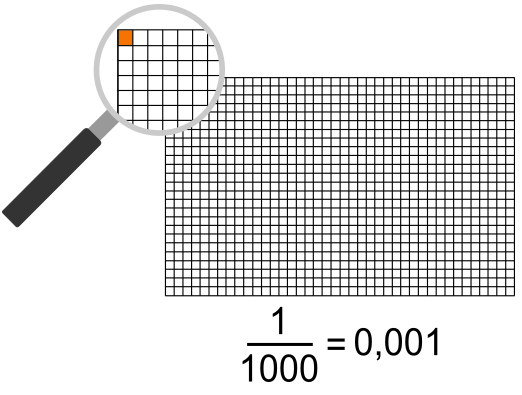
\includegraphics[width=.6\columnwidth]{img/millesimi1.png}
\end{figure}    

Dalla figura, possiamo capire che \alert{mille millesimi sono un'unità}.
\end{frame}



\section{Misura}


\begin{frame}
\frametitle{Perché misuriamo?}
L'operazione di misura è il confronto tra una quantità e una certa \alert{unità di misura}.\pause

~

È fondamentale misurare per:
\begin{itemize}
  \item poter \alert{confrontare} due quantità, cioè stabilire quale è la più grande;\pause
  \item poter \alert{comunicare} ad altre persone informazioni sulle quantità.
\end{itemize}
\end{frame}



\begin{frame}
\frametitle{Cosa misuriamo?}
Si possono misurare moltissime cose, come ad esempio:
\begin{itemize}
  \item l'altezza di una stanza ($  3,10 \, m $);
  \item la massa di una mela ($ 0,12  \, kg $);
  \item la durata di una partita ($  5400 \, s $);
  \item la velocità di un download ($  1024 \, kB/s $);
  \item lo spessore di un capello ($  0,00008 \, m $);
  \item la corrente che passa in un computer ($  1,5 \, A $);
  \item l'energia utilizzata da un phon ($ 3600  \, kJ $);
  \item la luminosità di una lampadina ($  2700 \, lumen $);
  \item la dimensione del baule di un'auto ($  235 \, L $);
  \item ecc.
\end{itemize}
\end{frame}


\begin{frame}
\frametitle{Come misuriamo?}
Per eseguire una misura, è sempre necessario uno \alert{strumento di misura}:
\begin{columns}
  \begin{column}{0.25\textwidth}
  \begin{figure}
    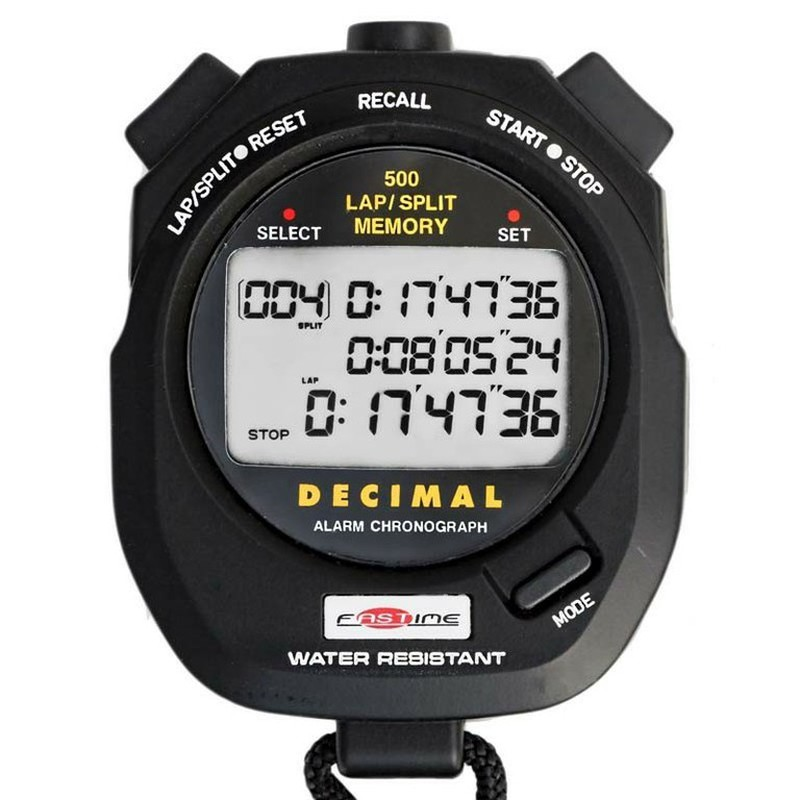
\includegraphics[width=\columnwidth]{img/cronometro.jpg}

    Cronometro
  \end{figure}    
  \end{column}
  \begin{column}{0.25\textwidth}
  \begin{figure}
    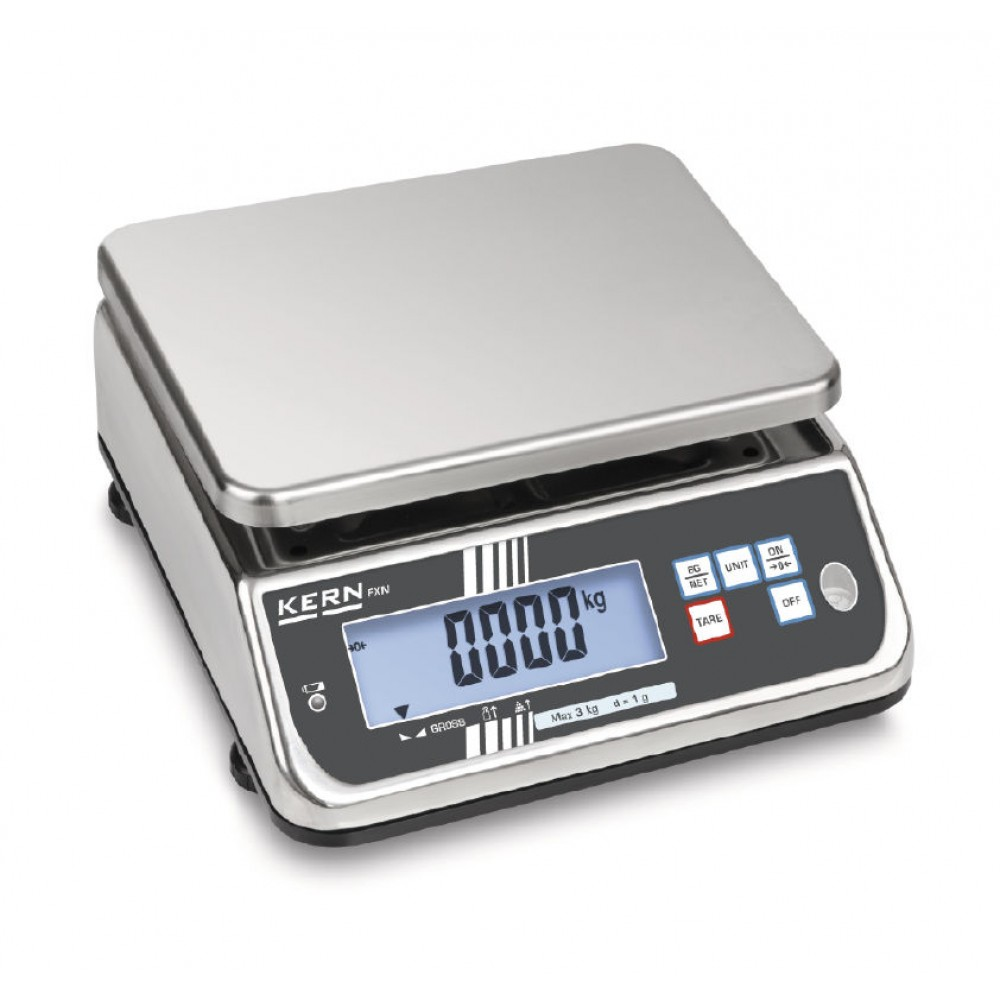
\includegraphics[width=\columnwidth]{img/bilancia.jpg}

    Bilancia
  \end{figure}    
  \end{column}
  \begin{column}{0.25\textwidth}
  \begin{figure}
    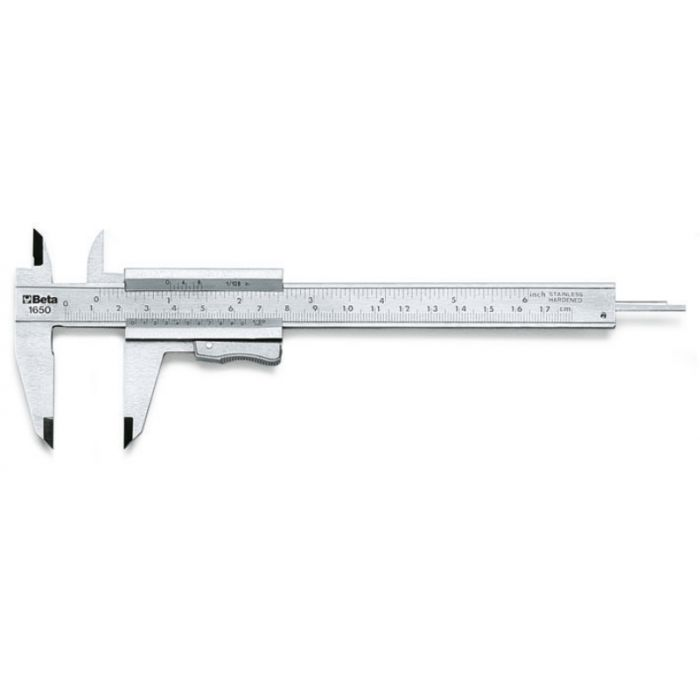
\includegraphics[width=\columnwidth]{img/calibro.jpg}

    Calibro
  \end{figure}    
  \end{column}
  \begin{column}{0.25\textwidth}
  \begin{figure}
    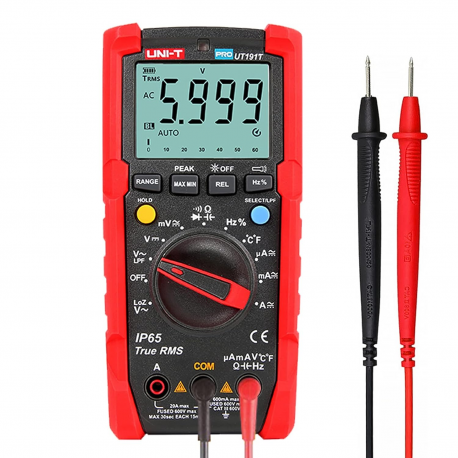
\includegraphics[width=\columnwidth]{img/multimetro.jpg}

    Multìmetro
  \end{figure}    
  \end{column}
\end{columns}\pause

~

~

\begin{itemize}
  \item Sensibilità = misura più piccola che lo strumento può eseguire;
  \item portata = misura più grande che lo strumento può eseguire.
\end{itemize}
\end{frame}



\begin{frame}
\frametitle{Esercizi sulla misurazione}
\begin{enumerate}
  \item Associa ad ogni quantità il corretto strumento di misura:
  \begin{multicols}{2}
    Quantità:
    \begin{itemize}
        \item durata del salto di un gatto;
        \item lunghezza di un dito;
        \item spessore di un cartoncino;
        \item tempo di cottura della pasta;
        \item altezza di un mobile;
        \item quantità di burro per una torta.
    \end{itemize}
    Strumenti:
    \begin{itemize}
      \item righello;
      \item metro;
      \item bilancia da cucina;
      \item cronometro;
      \item timer da cucina;
      \item calibro.
    \end{itemize}

    ~

    ~
  \end{multicols}
\end{enumerate}
\end{frame}





\section{Unità di misura}


\begin{frame}
\frametitle{Il Sistema Internazionale}
Le unità di misura sono delle quantità fisse, stabilite internazionalmente a partire dal 1791, per \alert{standardizzare la misura} nel mondo.\pause

~

Il \alert{Sistema Internazionale} delle unità di misura (1889) è costituito da \alert{7 unità di misura fondamentali}.\pause

~

\alert{Combinando le udm fondamentali possiamo ottenere delle udm derivate}, per misurare tutto ciò che è misurabile.
\end{frame}


\begin{frame}
\frametitle{Unità di misura fondamentali}
\begin{table}[htp]\centering
  \begin{tabular}{ccc}\hline\rule{0pt}{3ex}
        \textbf{Grandezza}    & \textbf{Udm}  & \textbf{Simbolo}\\\hline\rule{0pt}{3ex}
        lunghezza             & metro         & $ m $\\\hline\rule{0pt}{3ex}
        tempo                 & secondo       & $ s $\\\hline\rule{0pt}{3ex}
        massa                 & chilogrammo   & $ kg $ \\\hline\rule{0pt}{3ex}
        temperatura assoluta  & kelvin        & $ K $\\\hline\rule{0pt}{3ex}
        quantità di sostanza  & mole          & $ mol $\\\hline\rule{0pt}{3ex}
        corrente elettrica    & ampere        & $ A $\\\hline\rule{0pt}{3ex}
        intensità luminosa    & candela       & $ cd $\\\hline
  \end{tabular}
\end{table}
\end{frame}




\begin{frame}
\frametitle{Unità di misura derivate}
Ad esempio, misuriamo \alert{la superficie} (come quella di una pavimento) \alert{in $ m^2 $}:
\begin{center}
$ 1 \, m^2 = 1 \, m \cdot m $
\end{center}\pause

~

Misuriamo invece \alert{la potenza} (come quella del motore di un'auto o di una piastra per capelli) \alert{in Watt}:
\begin{center}
$ 1 \, W = 1 \, \dfrac{kg \cdot m^2}{s^3} $
\end{center}
\end{frame}




\begin{frame}
\frametitle{Unità di misura utili ma imprecise}
\begin{figure}
  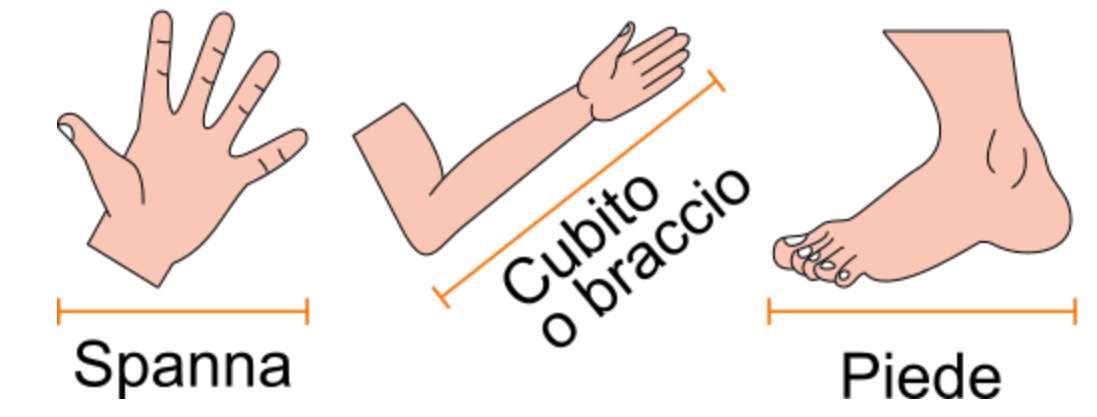
\includegraphics[width=\columnwidth]{img/spanna.png}
\end{figure}
\end{frame}






\begin{frame}
\frametitle{Le ``nostre'' unità di misura}
Nel nostro corso ci concentriamo sulle seguenti unità:

\begin{table}[]\def\arraystretch{1.5}
  \begin{tabular}{rcc}
  \textbf{Nome} & \textbf{Simbolo} & \textbf{Cosa misura} \\\hline
  metro         & m                & lunghezza            \\\hline
  litro         & L                & capacità, spazio     \\\hline
  grammo        & g                & massa                \\\hline
  secondo       & s                & tempo                \\\hline
  \end{tabular}
\end{table}
\end{frame}






\begin{frame}
\frametitle{Esercizi sulle unità di misura}
\begin{enumerate}
  \item Associa ad ogni quantità la corretta unità di misura:
  \begin{multicols}{2}
    Quantità:
    \begin{itemize}
        \item durata del salto di un gatto;
        \item lunghezza di un dito;
        \item contenuto di una lattina;
        \item spessore di un cartoncino;
        \item tempo di cottura della pasta;
        \item altezza di un mobile;
        \item dimensioni di una stanza;
        \item quantità di burro per una torta.
    \end{itemize}
    Unità di misura:
    \begin{itemize}
      \item secondi;
      \item litri;
      \item metri;
      \item grammi;
    \end{itemize}

    ~

    ~

    ~

    ~

    ~

  \end{multicols}
\end{enumerate}
\end{frame}




\section{Multipli}

\begin{frame}
\frametitle{Problemi di misura}
Come avrai notato da alcuni esempi, possiamo misurare cose \alert{molto grandi}, come la massa della Luna:

\[ 73.000.000.000.000.000.000.000 \, kg \]

~

oppure \alert{molto piccole}, come lo spessore di un capello:

\[ 0,00008 \, m \]\pause

~

Per rendere queste misure più comode da esprimere, esistono i \alert{multipli e sottomultipli delle unità di misura}.
\end{frame}





\begin{frame}
\frametitle{Multipli}
I multipli sono unità di misura 10, 100, 1000 volte più grandi di quella di partenza e vengono indicati con un prefisso:
\begin{itemize}
  \item \alert{da-} (deca-) per multipli \alert{10 volte più grandi};\pause
  
  \[ 1 \, daL = 10 \, L \]\pause
  \item \alert{h-} (etto-) per multipli \alert{100 volte più grandi};\pause
  
  \[ 1 \, hg = 100 \, g \]\pause

  \item \alert{k-} (chilo-) per multipli \alert{1000 volte più grandi}.\pause
  
  \[ 1 \, km = 1000 \, m \]
\end{itemize}
\end{frame}




\begin{frame}
\frametitle{Sottomultipli}
I sottomultipli sono unità di misura 10, 100, 1000 volte più piccole di quella di partenza e vengono indicati con un prefisso:
\begin{itemize}
  \item \alert{d-} (deci-) per sottomultipli \alert{10 volte più piccoli};\pause
  
  \[ 1 \, dL = 0,1 \, L \]\pause
  \item \alert{c-} (centi-) per sottomultipli \alert{100 volte più piccoli};\pause
  
  \[ 1 \, cm = 0,01 \, m \]\pause

  \item \alert{m-} (milli-) per sottomultipli \alert{1000 volte più piccoli}.\pause
  
  \[ 1 \, ms = 0,001 \, s \]
\end{itemize}
\end{frame}


\begin{frame}
\frametitle{Multipli e sottomultipli del metro}
Riassumendo, per il metro:
\begin{figure}
  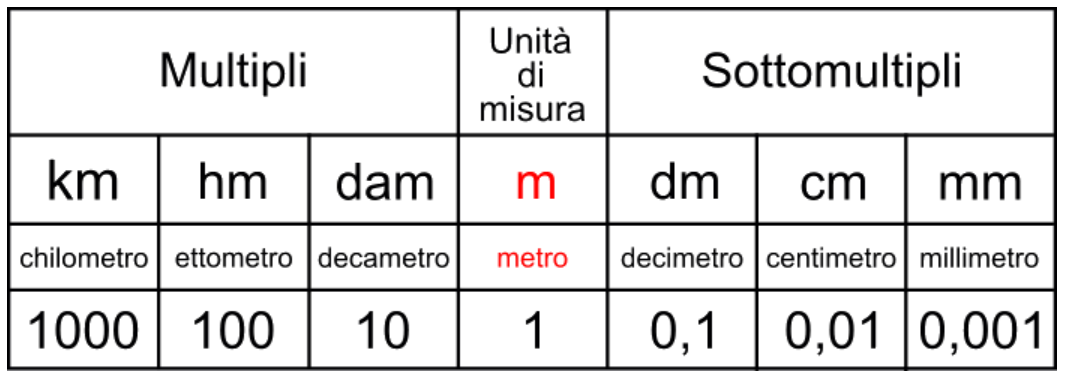
\includegraphics[width=\columnwidth]{img/metro.png}
\end{figure}
\end{frame}





\section{Equivalenze}



\begin{frame}
\frametitle{Equivalenze tra unità di misura}
Le equivalenze sono \alert{conversioni tra una udm all'altra}.

\[ 1,25 \, km = 1250 \, m \]\pause

~

Attenzione! Posso convertire solo unità \alert{dello stesso tipo}:\pause

\begin{itemize}
  \item posso convertire i grammi in chilogrammi;\pause
  \item \alert{non} posso convertire i grammi in secondi.
\end{itemize}
\end{frame}



\begin{frame}
\frametitle{Un'osservazione fondamentale}
\begin{columns}
  \begin{column}{0.5\textwidth}
  \begin{figure}
    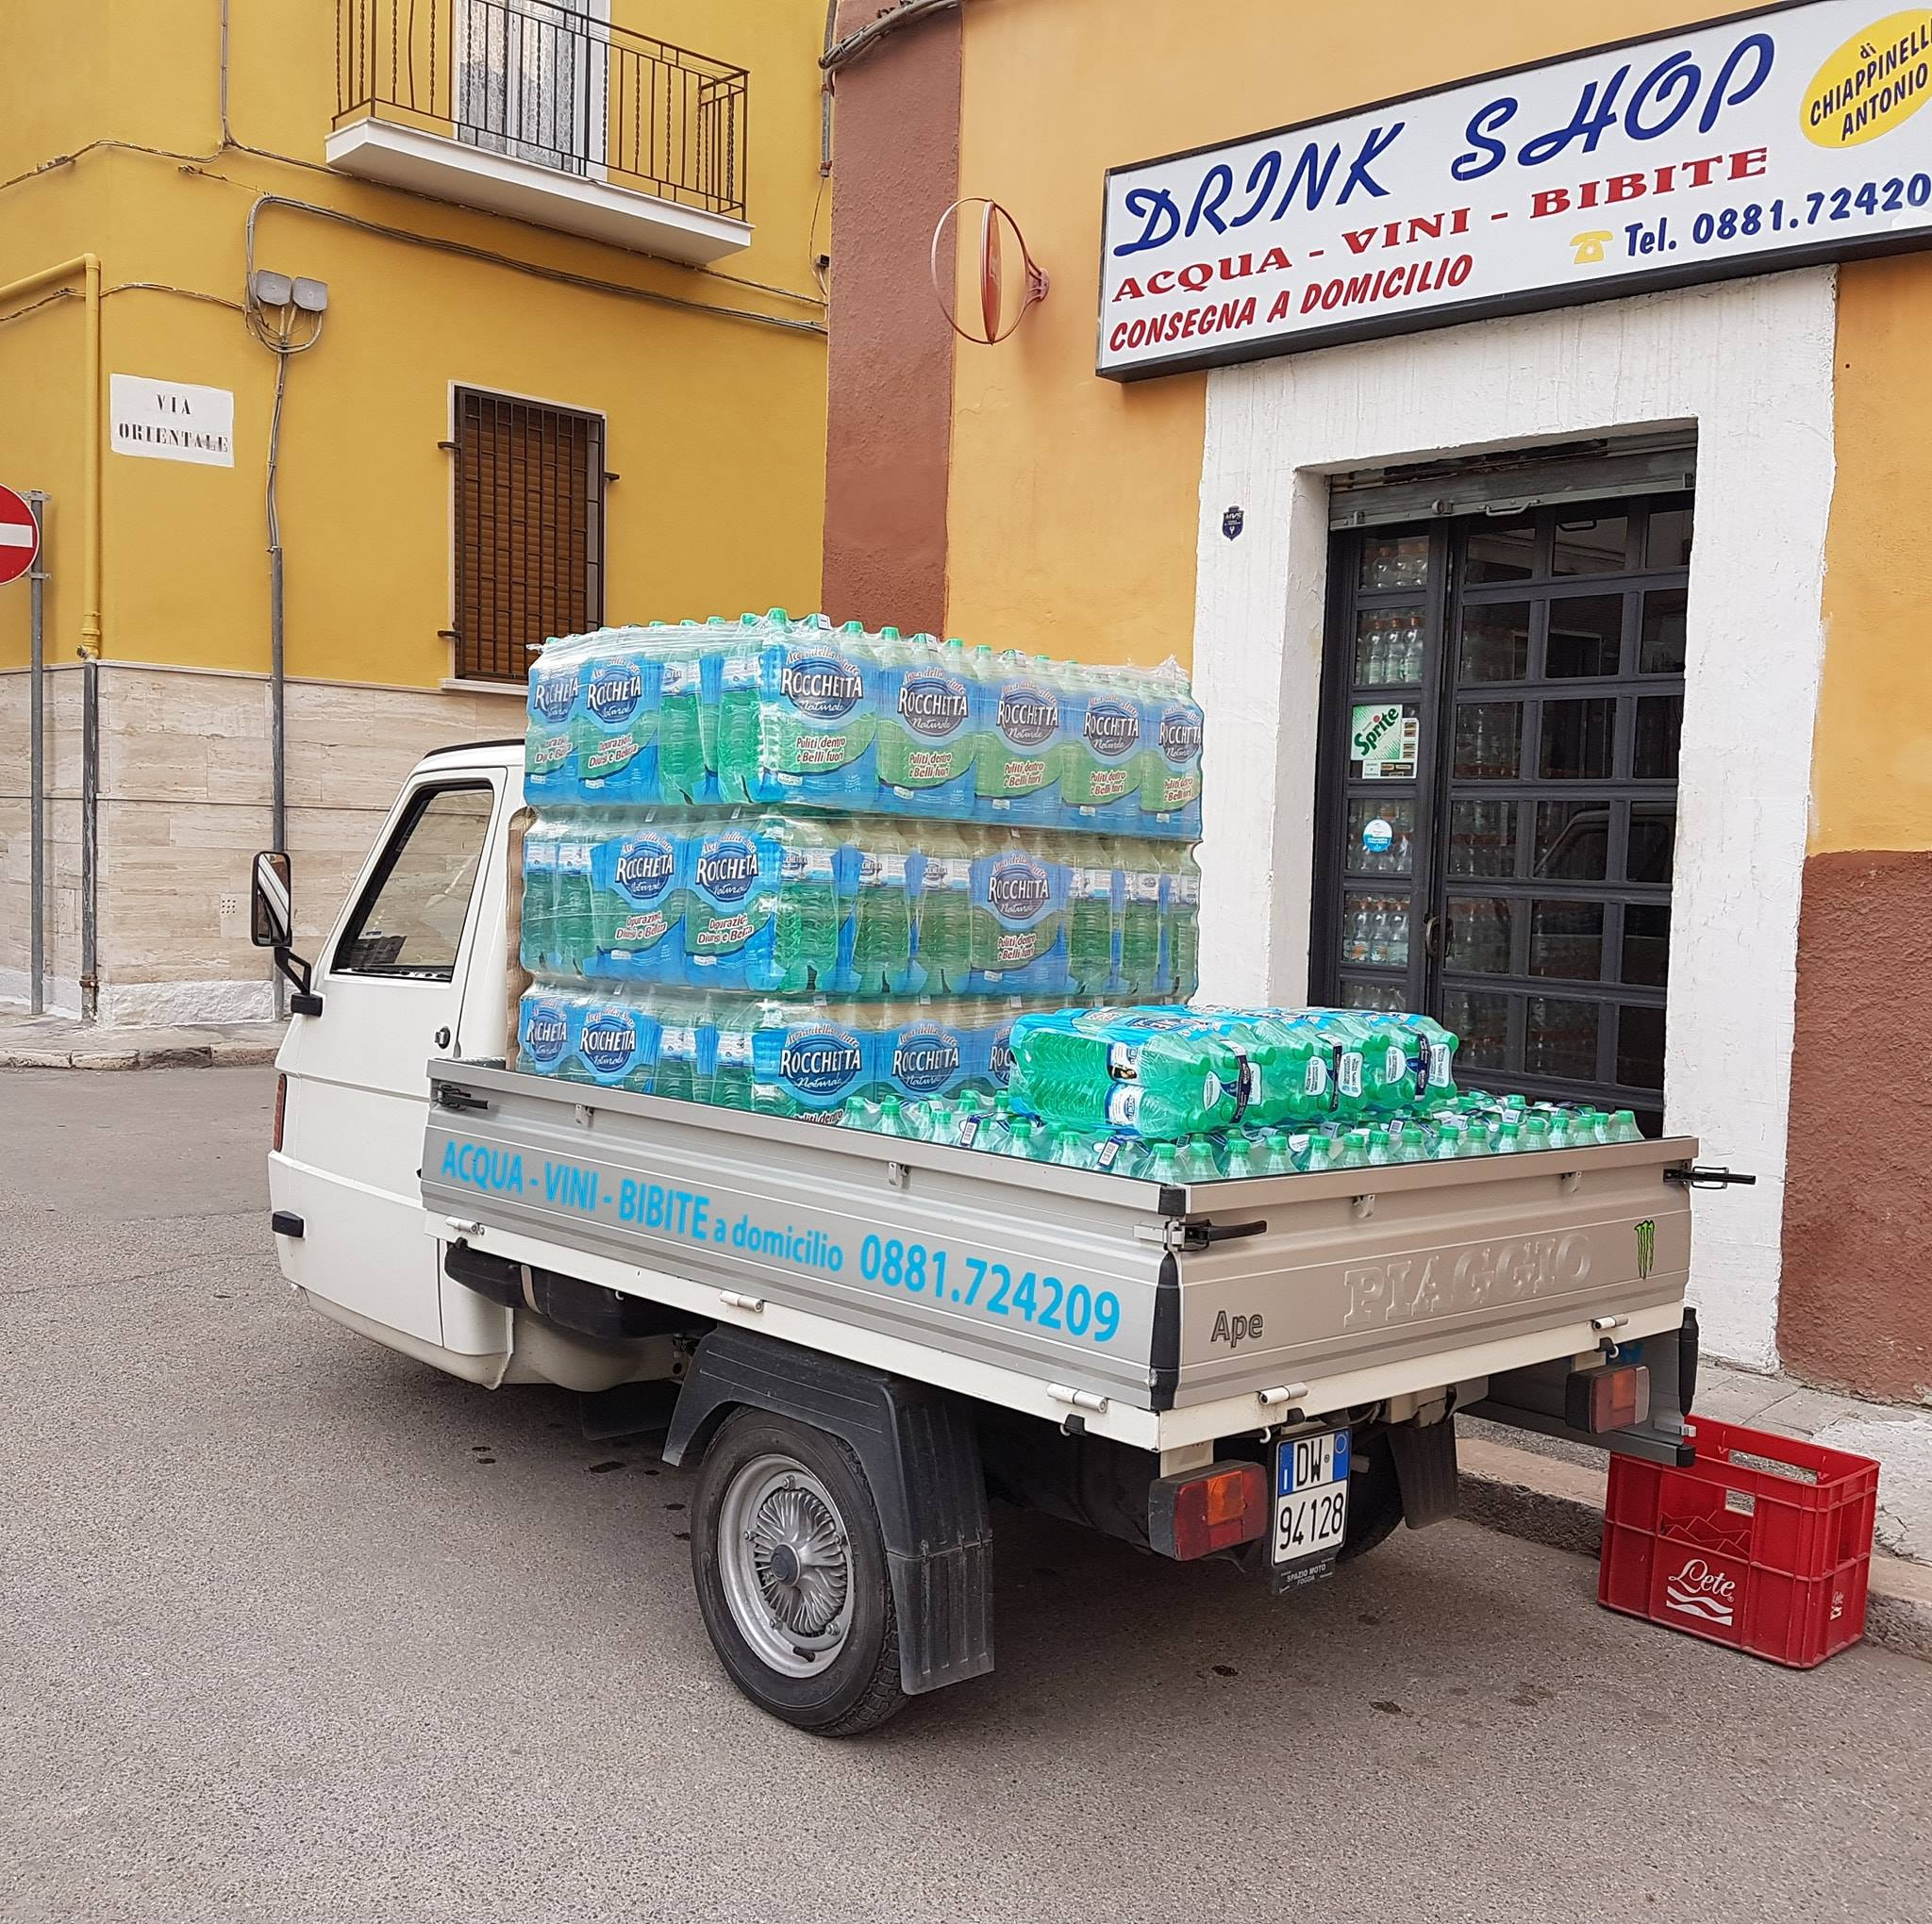
\includegraphics[width=\columnwidth]{img/bibite.jpg}
  \end{figure}    
  \end{column}
  \begin{column}{0.5\textwidth}
    Misuriamo in bottiglie:
    \begin{center}
      Ci sono \alert{$ 378 $} bottiglie d'acqua.\pause  
    \end{center}
    
    ~

    Misuriamo in casse:
    \begin{center}
      Ci sono \alert{$ 63 $} casse d'acqua.\pause  
    \end{center}
  \end{column}
\end{columns}

~


~

Se passiamo ad una ``unità di misura'' più grande, \alert{il numero diminuisce}!
\end{frame}




\begin{frame}
\frametitle{Funziona anche al contrario!}
\begin{columns}
  \begin{column}{0.5\textwidth}
  \begin{figure}
    
\includegraphics[width=\columnwidth]{img/biscotti.png}
  \end{figure}    
  \end{column}
  \begin{column}{0.5\textwidth}
    Misuriamo in pacchetti:
    \begin{center}
      Ci sono \alert{$ 7 $} pacchetti.\pause  
    \end{center}
    
    ~

    Misuriamo in biscotti:
    \begin{center}
      Ci sono \alert{$ 350 $} biscotti.\pause  
    \end{center}
  \end{column}
\end{columns}

~


~

Se passiamo ad una ``unità di misura'' più piccola, \alert{il numero aumenta}!
\end{frame}



\begin{frame}
\frametitle{Da grande a piccolo}
Quando passiamo ad una unità di misura \alert{più piccola}, il numero deve diventare \alert{più grande}:

\[ 120 \, m = 120.000 \, mm  \]\pause

Dobbiamo quindi ``spostare la virgola'' verso destra.
\end{frame}




\begin{frame}
\frametitle{Da piccolo a grande}
Quando passiamo ad una unità di misura \alert{più grande}, il numero deve diventare \alert{più piccolo}:

\[ 670 \, cL = 6,7 \, L  \]\pause

Dobbiamo quindi ``spostare la virgola'' verso sinistra.
\end{frame}



\begin{frame}
\frametitle{``Contare i salti''}
Come possiamo visualizzare \alert{di quanto} spostarci con la virgola?

~

Un esempio con i metri:

~

\begin{figure}
  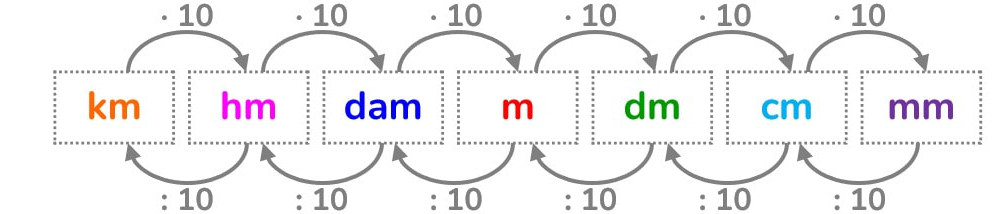
\includegraphics[width=\columnwidth]{img/saltimetro.jpg}
\end{figure}
\end{frame}


\begin{frame}
\frametitle{I ``salti'' con altre udm}
\begin{figure}
  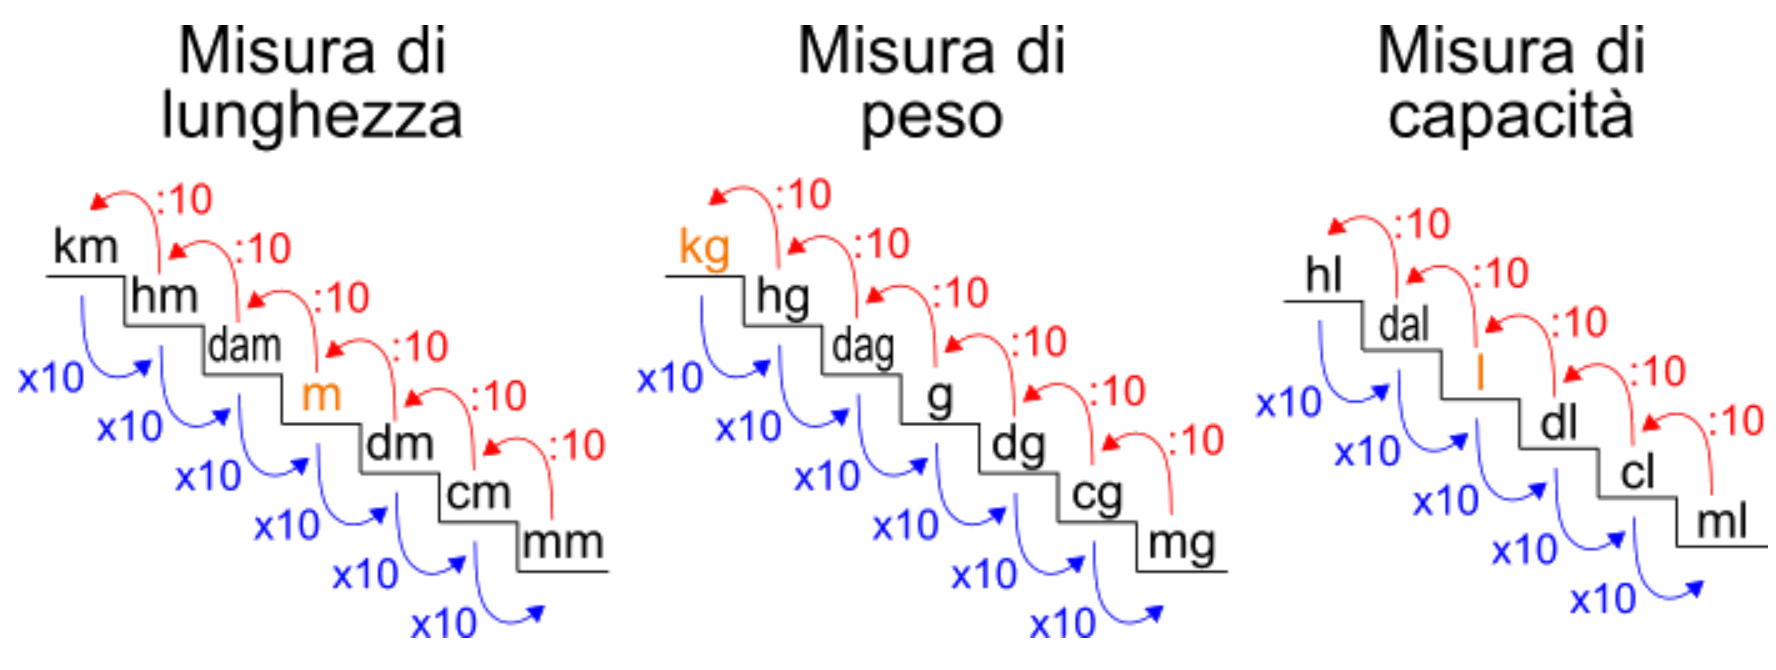
\includegraphics[width=\columnwidth]{img/saltiudm.png}
\end{figure}
\end{frame}


\begin{frame}
\frametitle{Esempio 1}
\[  1245 \, cm = \ldots \, m \]\pause

~

Come pensare:
\begin{enumerate}
  \item i metri sono più grandi dei centimetri, quindi:
  \item il numero diventa più piccolo, quindi:
  \item sposto la virgola a sinistra;
  \item tra cm e m ci sono due salti, quindi:
  \item la virgola si sposta a sinistra di due posti.
\end{enumerate}
  
\[  12\alert{\overleftarrow{45\phantom{,}}} \, cm = 12,45 \, m \]\pause
\end{frame}


\begin{frame}
\frametitle{Esempio 2}
\[  5,7 \, dL = \ldots \, mL \]\pause

~

Come pensare:
\begin{enumerate}
  \item i mL sono più piccoli dei dL, quindi:
  \item il numero diventa più grande, quindi:
  \item sposto la virgola a destra;
  \item tra dL e mL ci sono due salti, quindi:
  \item la virgola si sposta a destra di due posti (devo aggiungere degli zeri).
\end{enumerate}
  
\[  5\alert{\overrightarrow{,7\phantom{0}}} \, dL = 570 \, mL \]\pause
\end{frame}








\begin{frame}
\frametitle{Esercizi sulle equivalenze tra udm}
\begin{enumerate}\setcounter{enumi}{0}
  \item Converti le seguenti misure in metri:
  \begin{multicols}{2}
    \begin{itemize}
        \item $ 15,8 \, cm $
        \item $ 0,532 \, km $
        \item $ 54556 \, mm $
        \item $ 0,98 \, dm $
        \item $ 44,7 \, km $
        \item $ 2145 \, cm $
    \end{itemize}
  \end{multicols}
  \item Converti le seguenti misure in dL:
  \begin{multicols}{2}
    \begin{itemize}
        \item $ 15 \, mL $
        \item $ 12 \, L $
        \item $ 0,566 hL $
        \item $ 1993 \, cL $
    \end{itemize}
  \end{multicols}
  \item Converti le seguenti misure in g:
  \begin{multicols}{2}
    \begin{itemize}
        \item $ 12,5 \, kg $
        \item $ 1,34 \, hg $
        \item $ 5666 \, mg $
        \item $ 599,2 \, cg $
    \end{itemize}
  \end{multicols}
\end{enumerate}
\end{frame}


\begin{frame}
\frametitle{Esercizi sulle equivalenze tra udm}
\begin{enumerate}\setcounter{enumi}{3}
  \item Ricopia sul quaderno il seguente schema di un mobile, convertendo tutte le misure in millimetri:
  \begin{figure}
    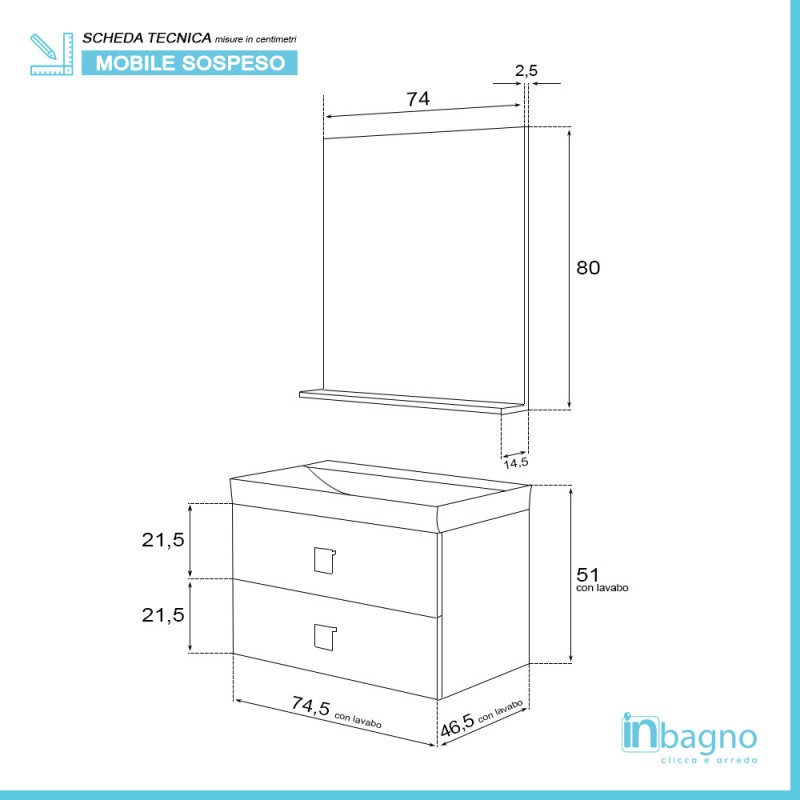
\includegraphics[width=.6\columnwidth]{img/mobile.jpg}
  \end{figure}
\end{enumerate}
\end{frame}






%MISURA LA POTENZA DEL PHON E DELLA PIASTRA!!!

%ESERCIZIO IN CUI SI CONVERTONO LE MISURE DI QUALCOSA (UNA STANZA, UN OGGETTO) DA UNA UDM ALL'ALTRA


\section{Unità derivate}


\begin{frame}
\frametitle{Altre unità}
Le unità che abbiamo possono essere \alert{combinate tra loro} per ottenerne delle altre.\pause

~

I multipli, sottomultipli e le conversioni con queste nuove unità funzionano \alert{esattamente come con quelle di base}.

\[ 1500 \, W = 1,5 \, kW \]

~

\[ 12 \, kcal = 12.000 \, cal\]
\end{frame}





\begin{frame}
\frametitle{Energia}
L'energia è quello che permette al nostro corpo e alle macchine che utilizziamo di funzionare.\pause

\begin{columns}
  \begin{column}{0.3\textwidth}
  \begin{figure}
    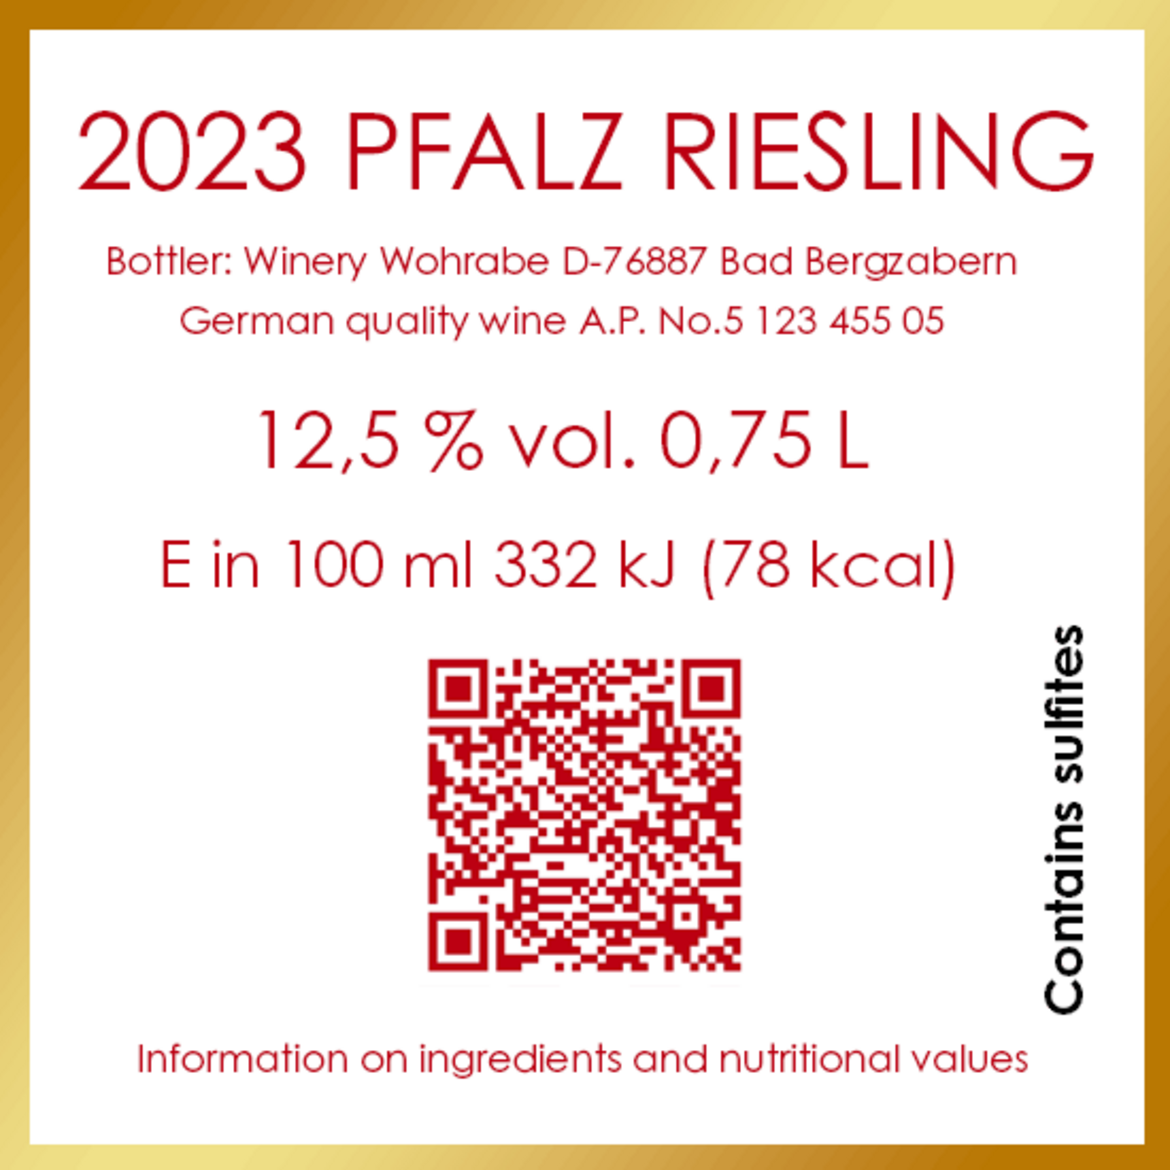
\includegraphics[width=\columnwidth]{img/etichetta.png}
  \end{figure}    
  \end{column}
  \begin{column}{0.3\textwidth}
  \begin{figure}
    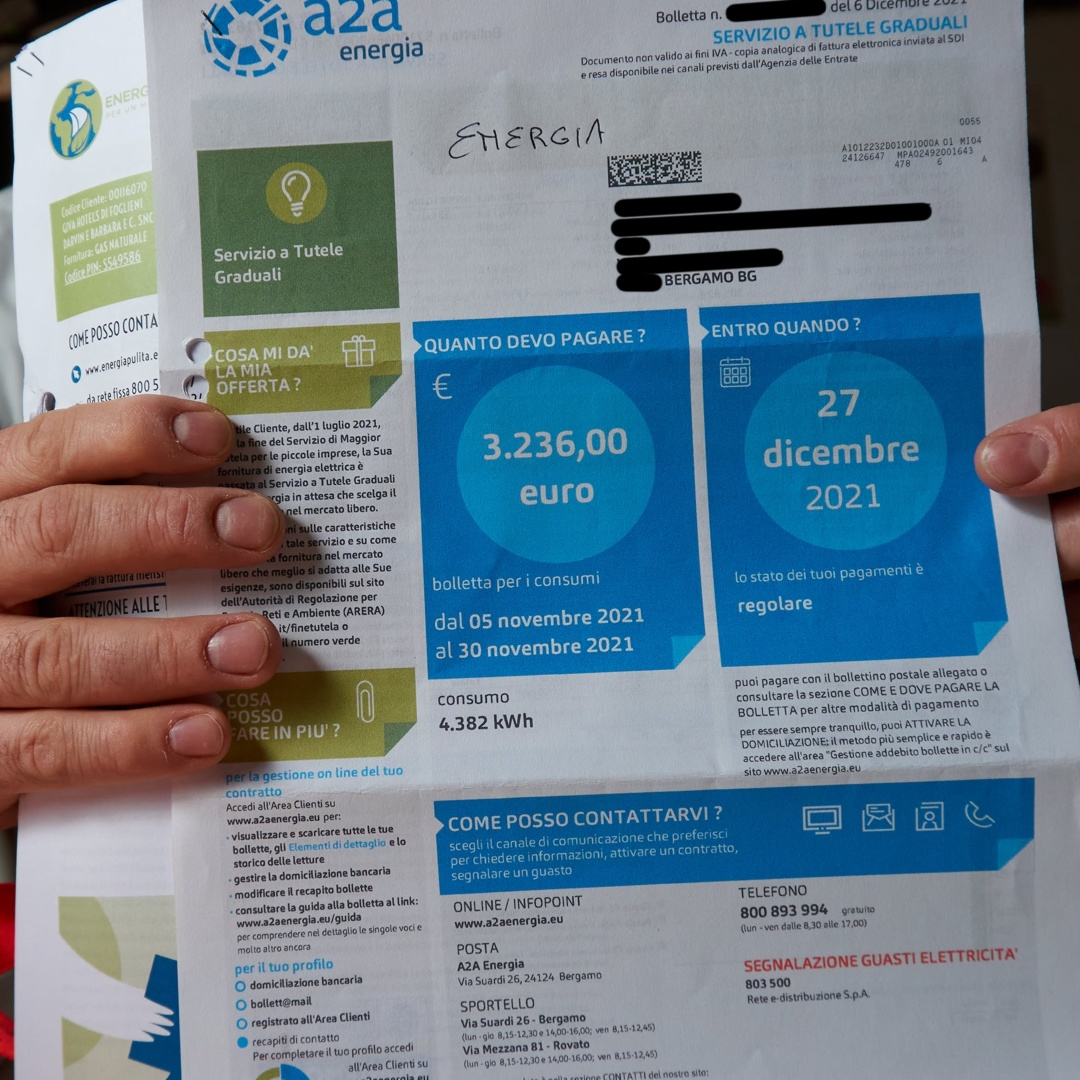
\includegraphics[width=\columnwidth]{img/bolletta.jpg}
  \end{figure}    
  \end{column}
\end{columns}

~

L'energia si misura in:
\begin{itemize}
  \item joule e kilojoule, $ J $ e $ kJ $;
  \item calorie e kilocalorie, $ cal $ e $ kcal $;
  \item kilowattora, $ kWh $, come nelle bollette (a ottobre 2024, $ 1 \, kWh  $ costa circa $ 0,13 $ €).
\end{itemize}
\end{frame}


\begin{frame}
\frametitle{Potenza}
La potenza indica quanta energia viene utilizzata/fornita al secondo.

~

La potenza si misura in:
\begin{itemize}
  \item watt e kilowatt, $ W $ e $ kW $;
  \item cavalli vapore, $ cv $ o $ hp $.
\end{itemize}

\begin{columns}
  \begin{column}{0.25\textwidth}
  \begin{figure}
    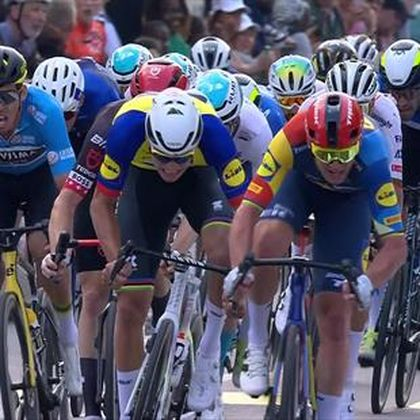
\includegraphics[width=\columnwidth]{img/ciclisti.jpg}

    $ 700 \, W $
  \end{figure}    
  \end{column}
    \begin{column}{0.25\textwidth}
  \begin{figure}
    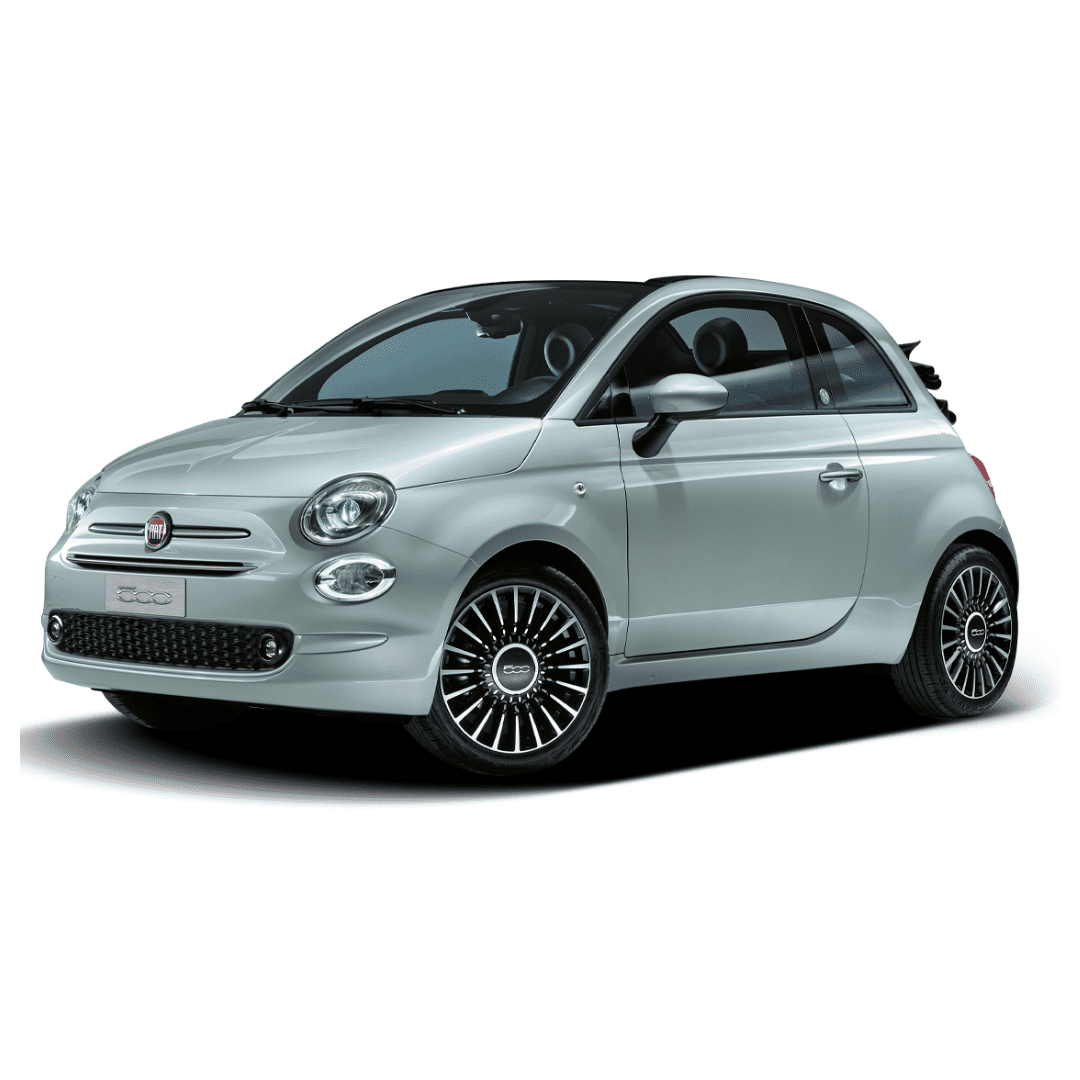
\includegraphics[width=\columnwidth]{img/500.png}

    $ 69 \, cv  = 51 \, kW $, 
  \end{figure}    
  \end{column}
  \begin{column}{0.25\textwidth}
  \begin{figure}
    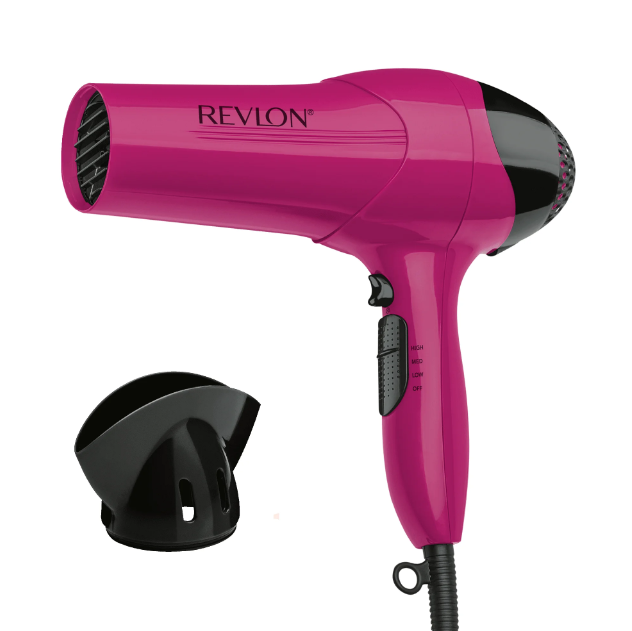
\includegraphics[width=\columnwidth]{img/phon.png}

    $ 1875 \, W $
  \end{figure}    
  \end{column}
  \begin{column}{0.25\textwidth}
  \begin{figure}
    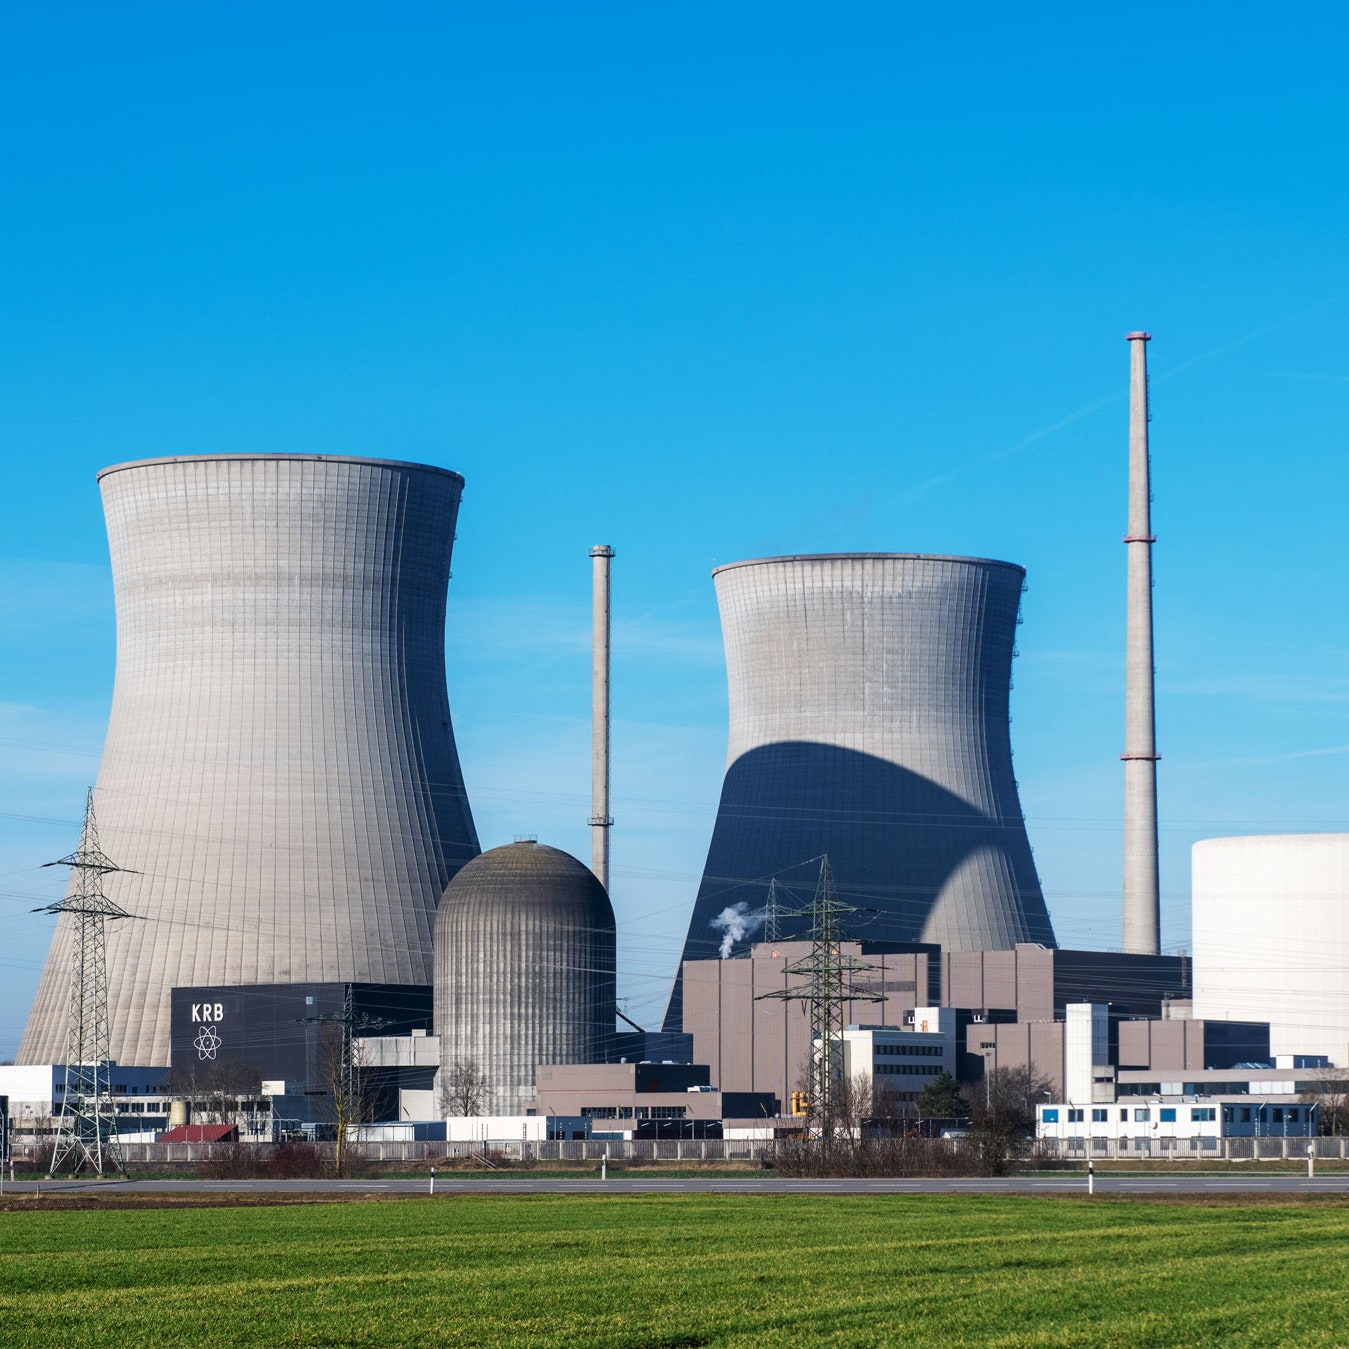
\includegraphics[width=\columnwidth]{img/centrale.jpg}

    $ > 600.000 \, kW $
  \end{figure}    
  \end{column}
\end{columns}
\end{frame}


\begin{frame}
\frametitle{Corrente elettrica}
La corrente elettrica è ciò che scorre nei cavi dei nostri dispositivi elettronici e delle nostre lampadine e si misura in ampere, $ A $.

\begin{columns}
  \begin{column}{0.3\textwidth}
  \begin{figure}
    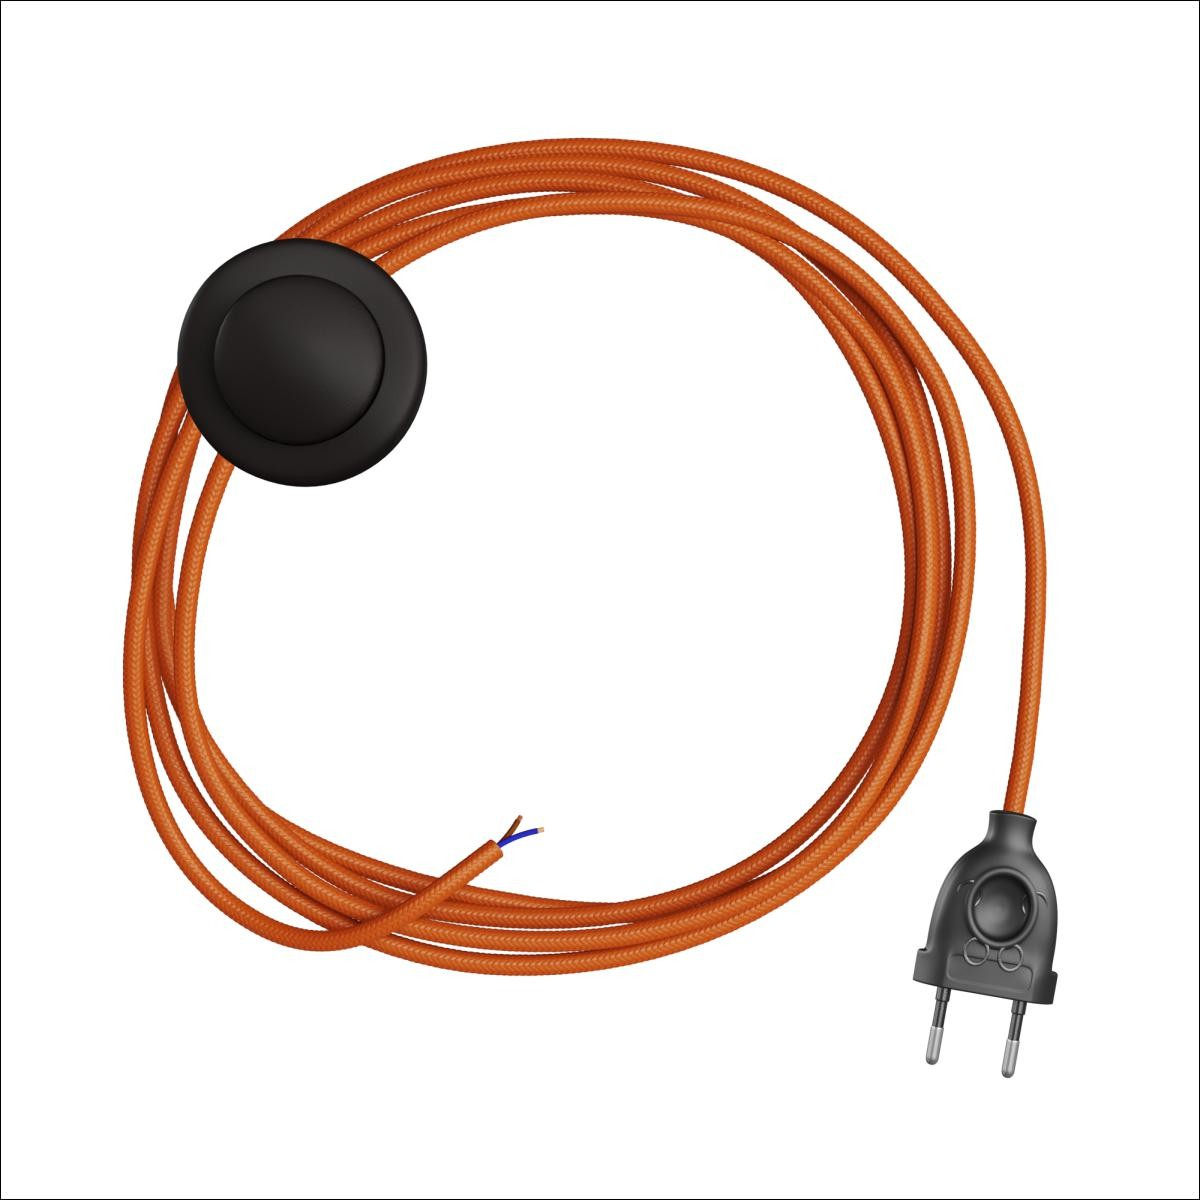
\includegraphics[width=\columnwidth]{img/cavo.jpg}

    $ 70 \, mA $
  \end{figure}    
  \end{column}
  \begin{column}{0.3\textwidth}
  \begin{figure}
    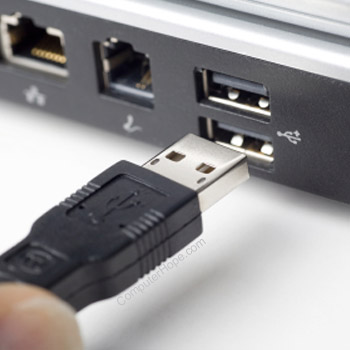
\includegraphics[width=\columnwidth]{img/usb.jpg}

    $ 0,5 \, A$
  \end{figure}    
  \end{column}
\end{columns}

~

Una corrente sopra i $ 10 \, mA $ può essere pericolosa per gli umani. Oltre i $ 200 \, mA $ si hanno effetti letali.
\end{frame}



\begin{frame}
\frametitle{Differenza di potenziale}
La differenza di potenziale o tensione si misura in volt ($ V $) ed è ciò che permette alla corrente di scorrere. Quando premiamo un interruttore stiamo attivando una tensione nel cavo.

~

\begin{columns}
  \begin{column}{0.3\textwidth}
  \begin{figure}
    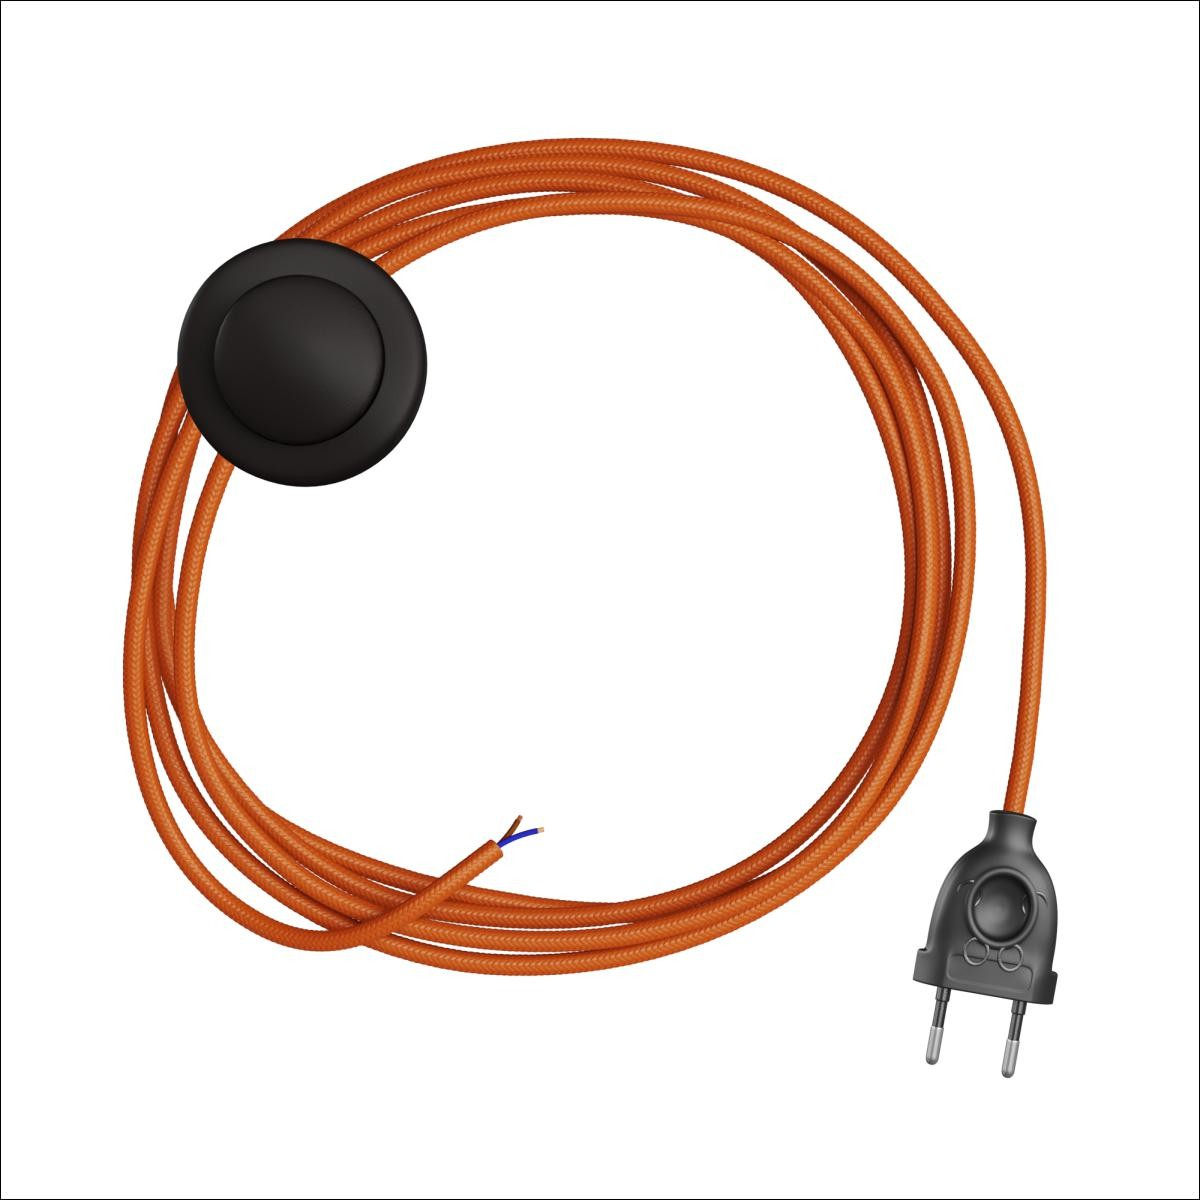
\includegraphics[width=\columnwidth]{img/cavo.jpg}

    $ 220 \, V $ (AC)
  \end{figure}    
  \end{column}
  \begin{column}{0.3\textwidth}
  \begin{figure}
    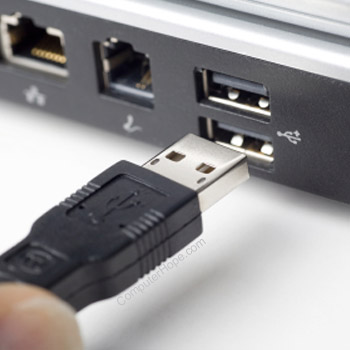
\includegraphics[width=\columnwidth]{img/usb.jpg}

    $ 5 \, V $ (DC)
  \end{figure}    
  \end{column}
  \begin{column}{0.3\textwidth}
  \begin{figure}
    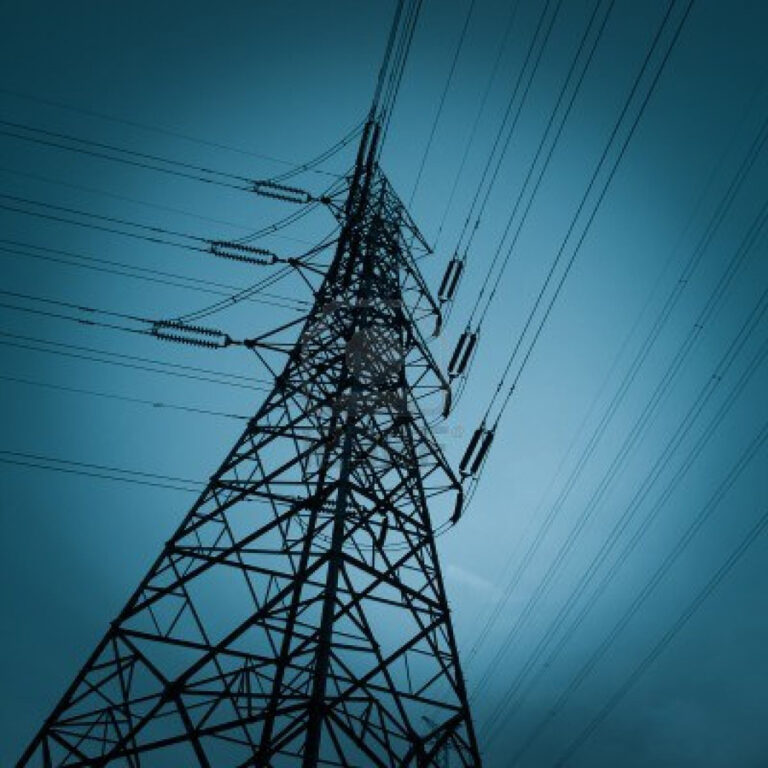
\includegraphics[width=\columnwidth]{img/altatensione.jpg}

    $ 50 \, kV $ (AC/DC)
  \end{figure}    
  \end{column}
\end{columns}

~

~


Se la tensione continua/alternata supera i $ 50 \, V/120 \, V $, la corrente può attraversare il corpo umano.
\end{frame}





\begin{frame}
\frametitle{Campo magnetico}
Il campo magnetico è l'effetto di una calamita intorno a sé e si misura in tesla ($ T $).

\begin{columns}
  \begin{column}{0.3\textwidth}
  \begin{figure}
    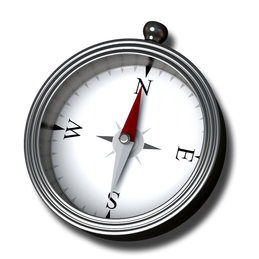
\includegraphics[width=\columnwidth]{img/bussola.png}

    $ 0,050 \, mT $
  \end{figure}    
  \end{column}
  \begin{column}{0.3\textwidth}
  \begin{figure}
    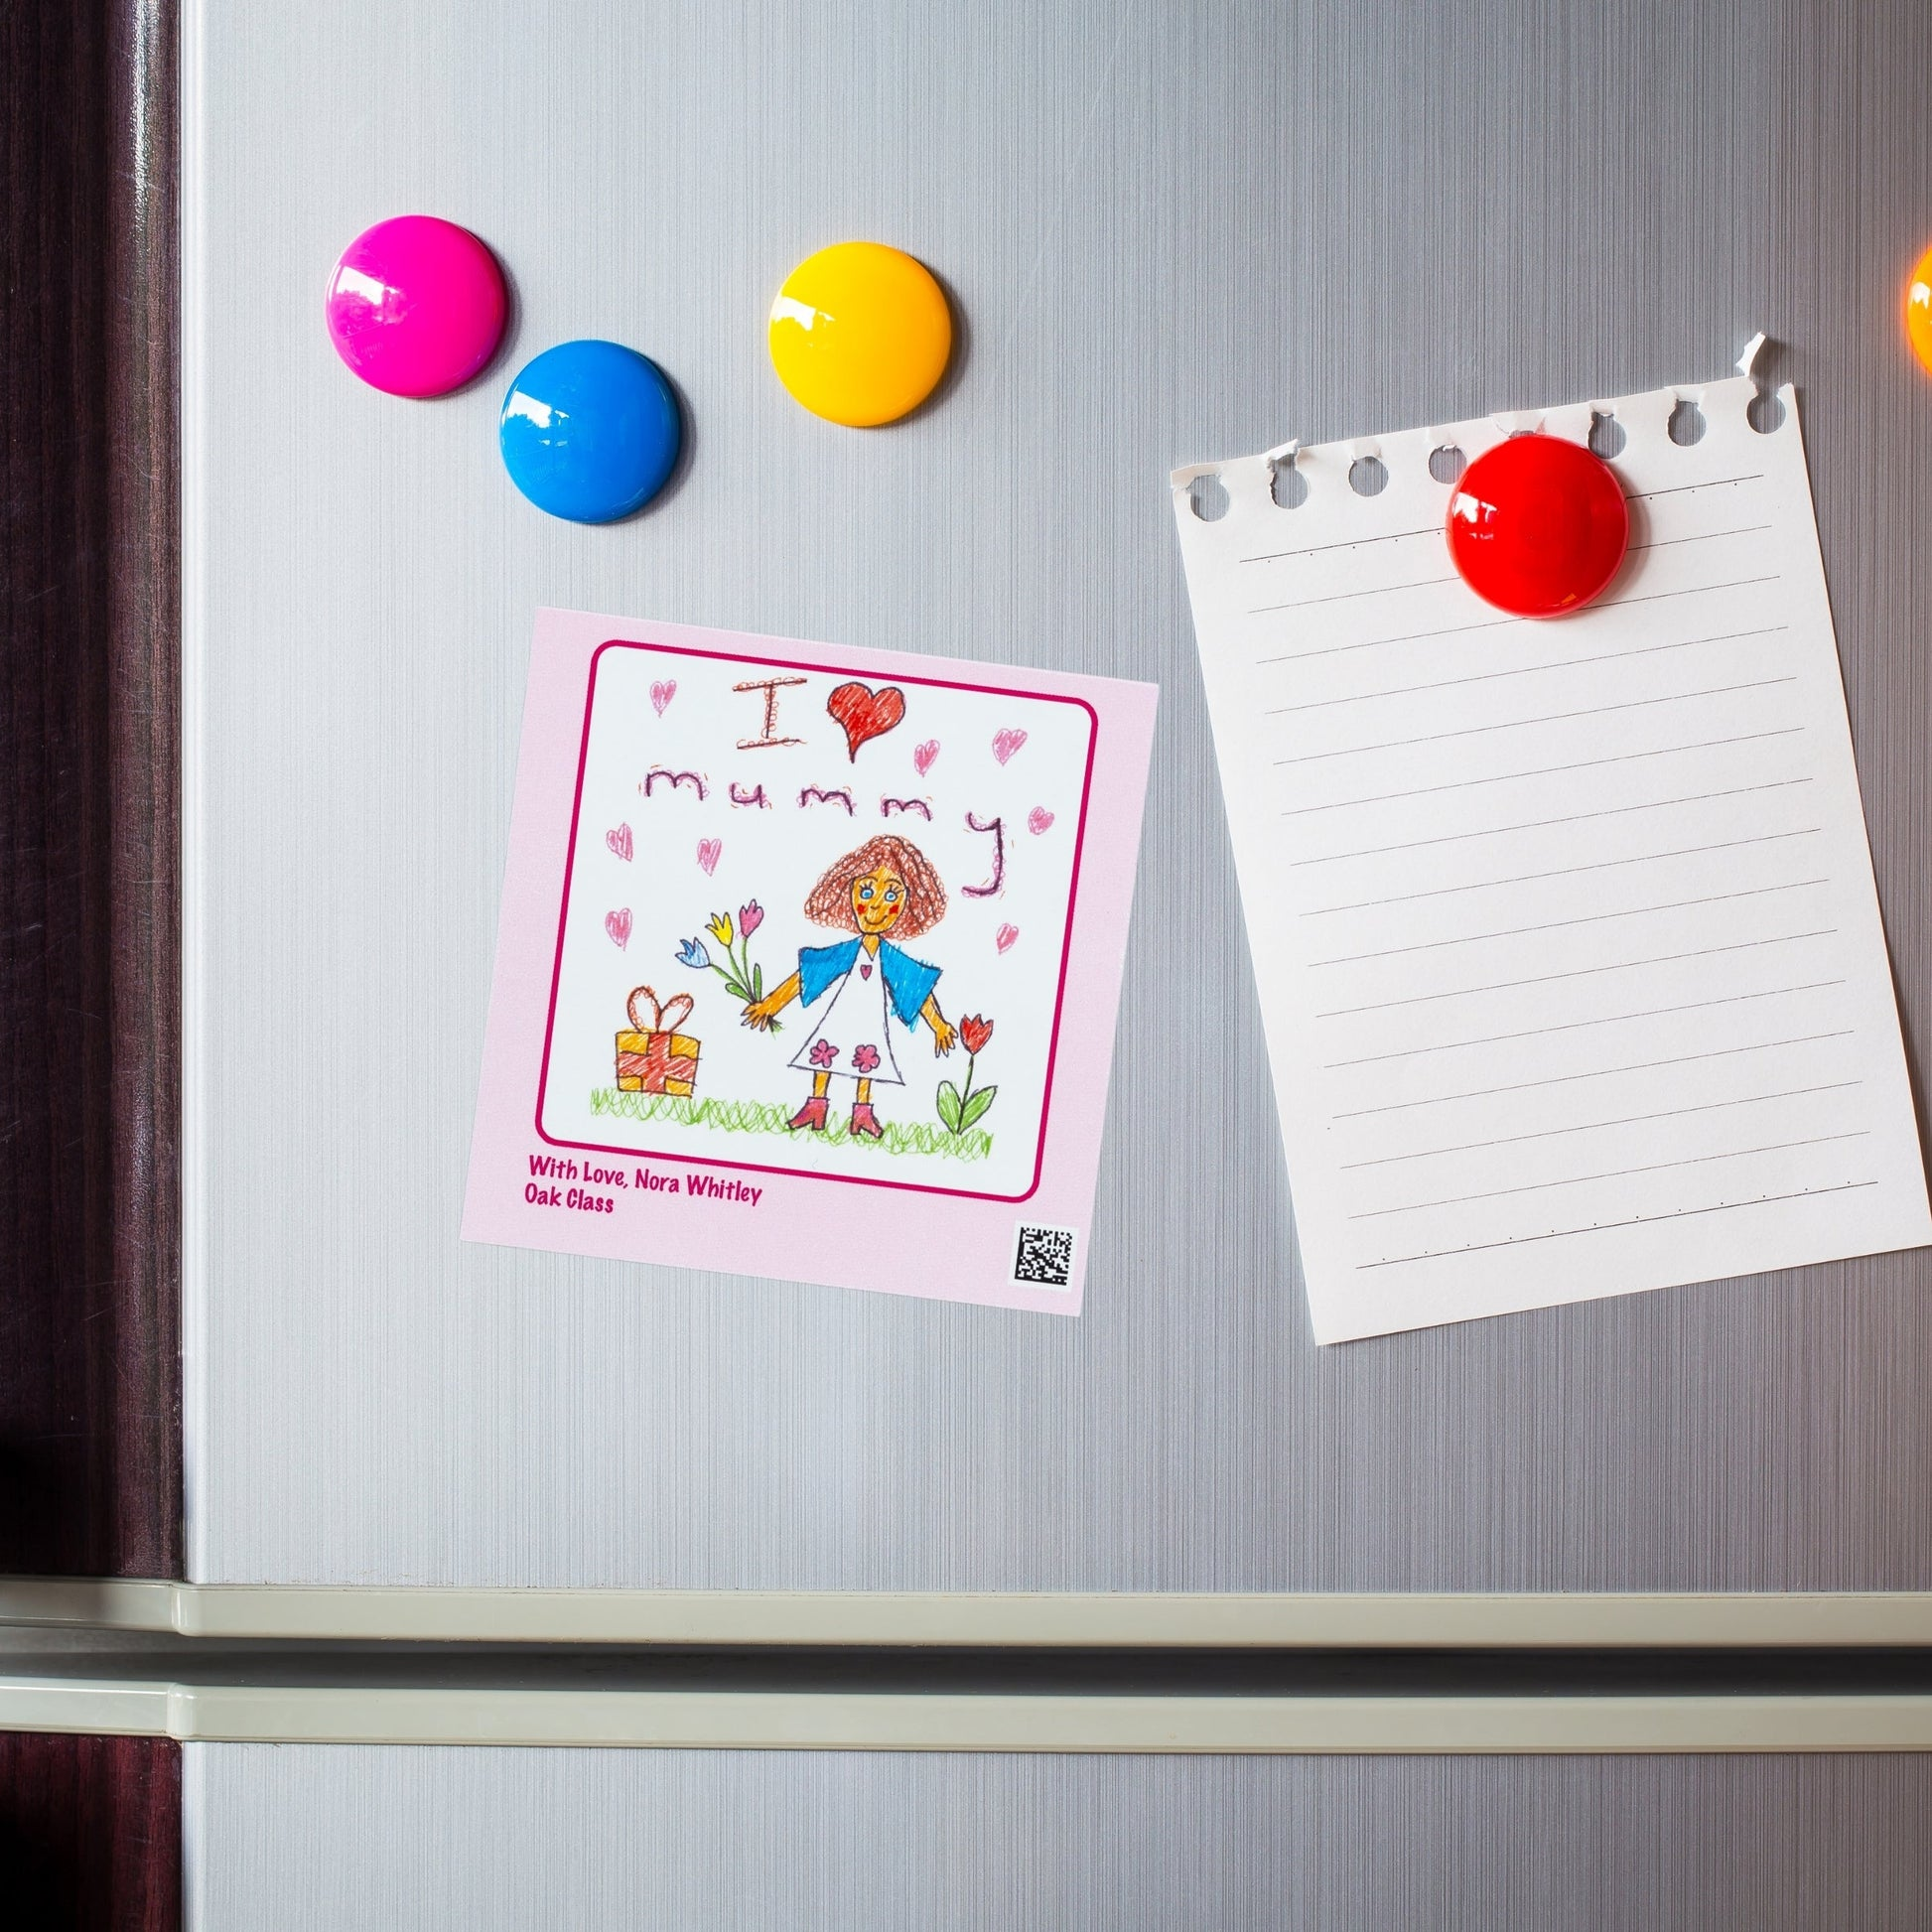
\includegraphics[width=\columnwidth]{img/frigo.jpg}

    $ 6 \, mT $
  \end{figure}    
  \end{column}
  \begin{column}{0.3\textwidth}
  \begin{figure}
    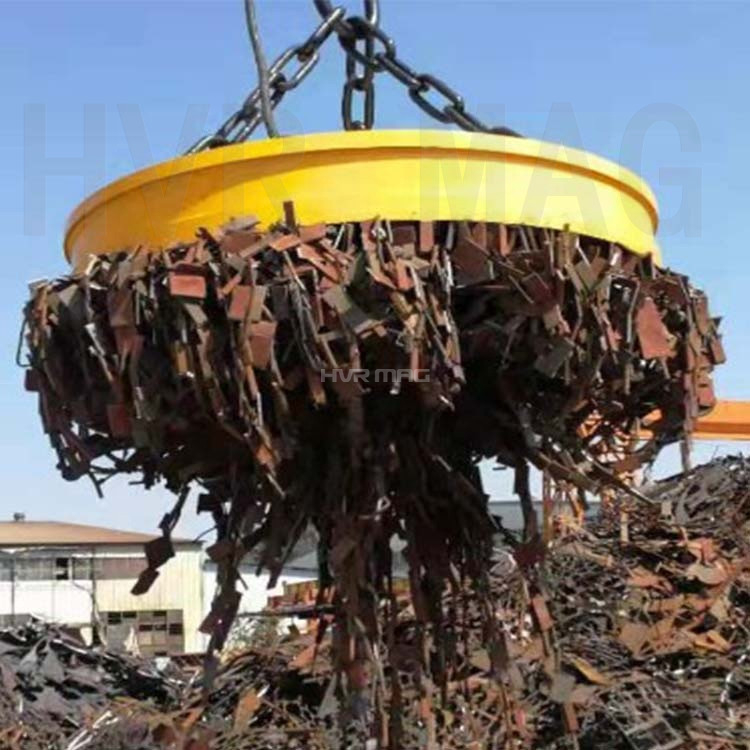
\includegraphics[width=\columnwidth]{img/scrap.jpg}

    $ 2 \, T $
  \end{figure}    
  \end{column}
\end{columns}
\end{frame}



\begin{frame}
\frametitle{Volume di un suono}
Il volume di un suono si misura in decibel ($ dB $). Volumi quotidiani oltre $ 85 \, dB $ sono dannosi.

\begin{figure}
  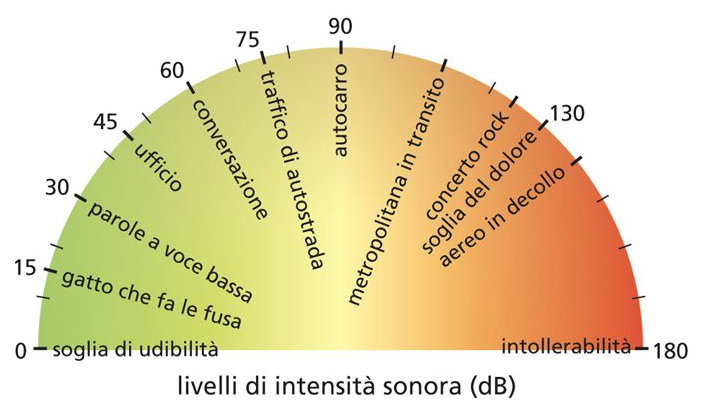
\includegraphics[width=.8\columnwidth]{img/volume.png}
\end{figure}

Gli auricolari moderni possono anche superare i $ 100 \, dB $.
\end{frame}






\end{document}
